\documentclass[11pt, openany, a5paper]{memoir}

\usepackage[utf8]{inputenc}
\usepackage[T1]{fontenc}
\usepackage{fourier}
\usepackage[indonesian]{babel}
\usepackage{microtype}
\usepackage{geometry}
\usepackage{lettrine}
\usepackage{pdfpages}

\geometry{
  paperwidth=148mm,
  paperheight=210mm,
  top=30mm,
  bottom=25mm,
  left=25mm,
  right=25mm,
  headheight=15pt,
  headsep=15pt
}

\nopartblankpage
\captiontitlefont{\normalfont}
\let\cleardoublepage\clearpage

\makechapterstyle{cerpenestetis}{%
  \chapterstyle{default}
  \renewcommand{\printchaptername}{}
  \renewcommand{\printchapternum}{}
  \renewcommand{\afterchapternum}{}
  \renewcommand{\chaptitlefont}{\normalfont\Huge\centering\scshape}
}
\chapterstyle{cerpenestetis}

\makepagestyle{estetis}
\makeevenhead{estetis}{\thepage}{}{\small\scshape Labirin Pikiran 25}
\makeoddhead{estetis}{\small\scshape\leftmark}{}{\thepage}
\makeevenfoot{estetis}{}{}{}
\makeoddfoot{estetis}{}{}{}
\pagestyle{estetis}

\usepackage{indentfirst}
\setlength{\parindent}{2.5em}
\setlength{\parskip}{0ex}

\newcommand{\penulis}[1]{%
  \nopagebreak
  \vspace{-1.2em}%
  \begin{center}%
    {\large\itshape Oleh #1}\\[0.5em]%
    \rule{2.5cm}{0.4pt}%
  \end{center}%
  \vspace{1.5em}%
}

\newcommand{\awalcerpen}[2]{%
  \lettrine[lines=3, findent=2pt]{#1}{#2}%
}

\newcommand{\jedacerita}{%
  \fancybreak{\vspace{0.8em}\textasteriskcentered\quad\textasteriskcentered\quad\textasteriskcentered\vspace{0.8em}}%
}

\newcommand{\jedahias}{%
  \fancybreak{\vspace{0.8em}$\diamondsuit\quad\diamondsuit\quad\diamondsuit$\vspace{0.8em}}%
}

\newcommand{\batin}[1]{{\itshape #1}}

\newcommand{\catatanpenulis}[1]{%
  \par\vspace{1.5em}%
  \noindent\rule{\linewidth}{0.2pt}\\[0.5em]%
                {\small\itshape #1}\par%
}

\begin{document}

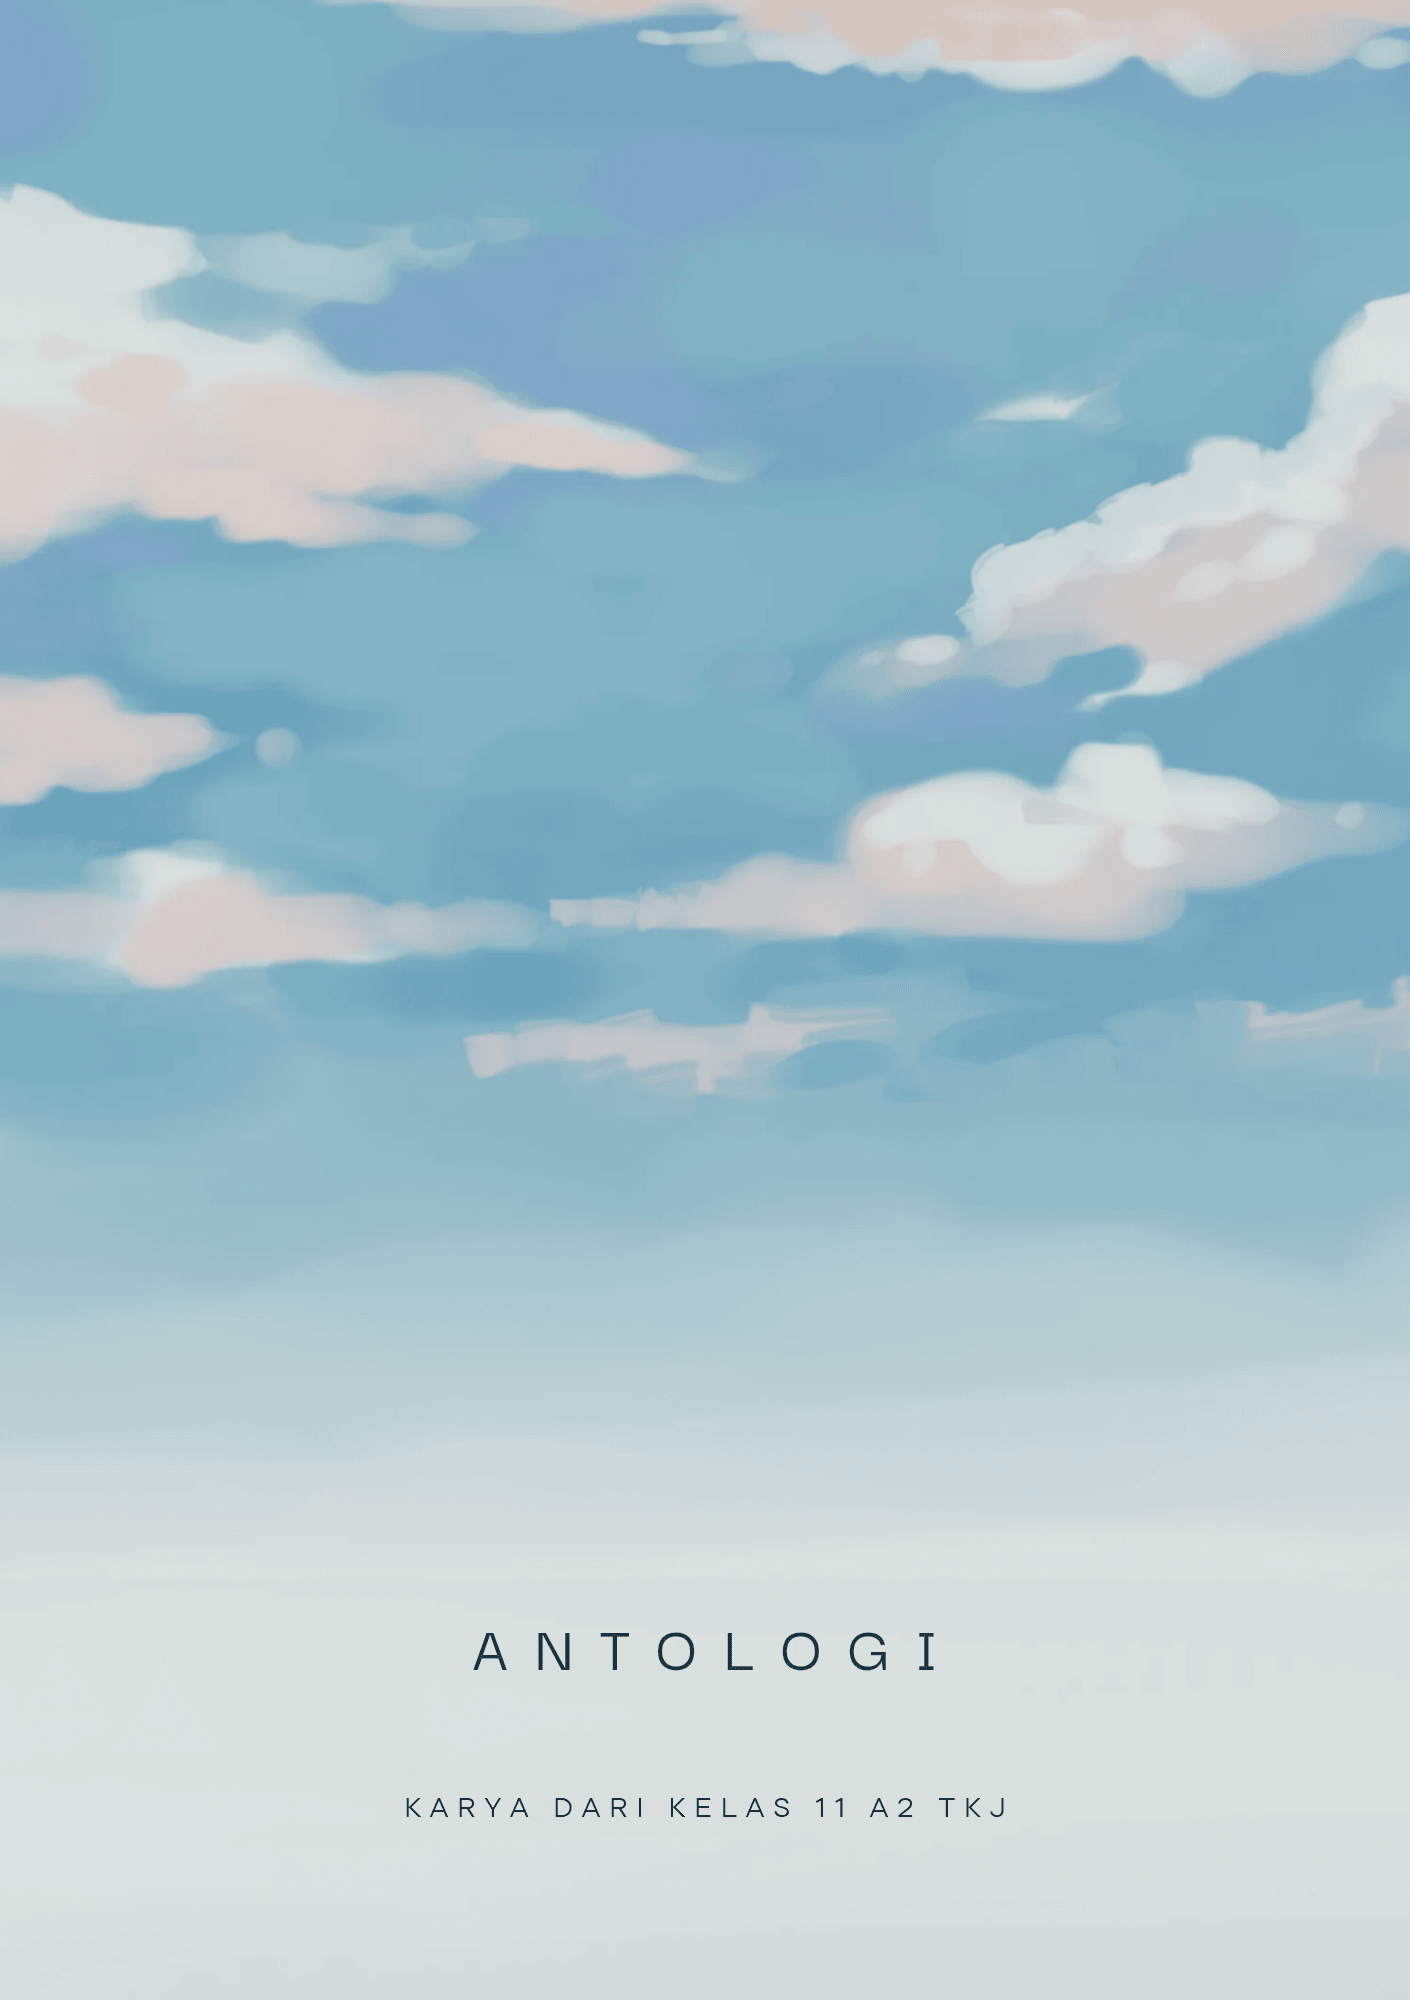
\includepdf[pages=1, scale=1, templatesize={\paperwidth}{\paperheight}, keepaspectratio=false, pagecommand={\thispagestyle{empty}}]{cover.png}

\thispagestyle{empty}
\begin{center}
  \vfill
      {\Large\scshape Tugas ASTS Kelas XI A2 TKJ} \\[0.5cm]
      \rule{\linewidth}{1pt} \\[0.8cm]
           {\Huge\bfseries LABIRIN PIKIRAN DUA PULUH LIMA} \\[0.5cm]
           {\large\itshape Antologi Cerpen Bersama} \\[0.8cm]
           \rule{\linewidth}{1pt} \\
           \vfill
               {\small\scshape Editor:}\\
               {\large Wisam Yassar Mahardika}
               \vfill
               \vfill
                   {\small\scshape \today}
                   \vspace*{1cm}
\end{center}
\clearpage

\frontmatter
\pagestyle{plain}

\chapter*{Kata Pengantar}
\addcontentsline{toc}{chapter}{Kata Pengantar}

Puji dan syukur kami panjatkan ke hadirat Tuhan Yang Maha Esa, karena atas rahmat-Nya, buku antologi cerpen berjudul \textit{Labirin Pikiran Dua Puluh Lima} ini dapat diselesaikan dengan baik. Buku ini merupakan wadah kreativitas bagi para penulis untuk menuangkan gagasan, emosi, dan imajinasi mereka ke dalam kisah kisah pendek yang bermakna.


Terima kasih yang sebesar-besarnya saya sampaikan kepada guru bahasa indonesia yang telah memberi wawasan, serta para penulis yang bekerja keras agar bisa menyampaikan cerita yang bermakna. Selamat membaca.

\vspace{2em}
\begin{flushright}
  Bandung, \today \\
  \vspace{1.5em}
  \textbf{Editor}
\end{flushright}
\clearpage

{
  \renewcommand{\contentsname}{\normalfont\Huge\centering\scshape Daftar Isi}
  \tableofcontents*
}
\clearpage

\mainmatter
\pagestyle{estetis}

\phantomsection
\chapter*{Just Friend}
\addcontentsline{toc}{section}{Just Friend --- Reka Rizki Pradana}
\penulis{Reka Rizki Pradana}

\awalcerpen{S}{uatu pagi disebuah sekolah}, Raka terlihat tidur diatas meja diiringi berisiknya kelas di jam itu. Hanya satu dipikiran Raka saat ini, yaitu Pulang, alih alih memikirkan percintaan seperti teman temannya, yang ia pikirkan hanya ingin segera meluluskan sekolahnya lalu mendapat penghasilan. Tetapi hari itu terasa berbeda bagi Neira, seorang perempuan kelas sebelah yang selalu terlihat ceria dan energik. 


Tiba tiba, meja Raka digebrak pelan ``Ka, masih pagi loh ini, udah ngantuk aja, semalem ngapain aja lo?'' kata Dimas, teman sebangku Raka, ``Apasih, kan belum bel dim!, Santai aja kali.'' Ucap Raka, Dimas terkejut, tak seperti biasanya Raka menjawab dengan nada seperti itu, ``Lo kenapa ka?, Ada masalah ya? Apa gara gara lo gagal deketin cewe?'' ucap Dimas ke Raka dengan nada kebingungan. ``Pikiran lo aja tuh cewe semua, buat apa juga gua deketin cewe, cuma bisa bikin cape doang.'' Jawab Raka sambil berdiri dari kursinya. Tak lama, Bel terdengar dan menandakan kegiatan membaca Quran di mushola akan segera dimulai.


Raka berjalan melewati lorong sekolah dengan tatapan kosong tanpa melihat kekiri dan ke kanan sedikit pun, Tak berselang lama, Neira memanggil Raka dari belakang. ``Raka!'' ucap Neira. ``Kenapa?'' jawab Raka dengan nada dingin sambil menoleh kebelakang. ``Nanti sore jangan dulu pulang ya, kumpul dulu eskul musik!'' Kata Neira, Raka tak menjawab apapun dan pergi meninggalkan Neira tanpa sepatah kata pun. Hanya satu yang ada diotak Raka saat itu, Pulang.


Setelah mengikuti seluruh kegiatan pembelajaran di Sekolah, Raka pun bersemangat untuk pulang, namun Neira sudah mengetahui bahwa Raka tidak akan mengikuti kumpul Ekskul.


``Akhirnya pulang juga.'' Kata Raka sambil berjalan keluar kelas, ``Mau kemana Ka?, Kumpul dulu.'' Dihadangnya Raka didepan pintu kelasnya oleh Neira. Alih alih melawan seperti biasanya, Raka malah memilih untuk menturuti apa yang Neira perintah, ``Iya iya ini juga mau ra, ngapain sih lo pake ngehadang hadang segala.'' Kata Raka, ``Ya biar lo ga kabur lah!, gua udah tau ya lo bakalan kabur.'' Jawab Neira.


Sesampainya diruangan di lantai 3, Mereka langsung bergabung bersama teman teman lainnya untuk mengikuti kumpul ekskul, tanpa Neira ketahui, ternyata dia baru saja menarik perhatian dari Raka, seorang yang tidak terlalu perduli dengan percintaan.


``Eh pulangnya bikin video dulu yuk!'' Kata Neira ke teman teman yang lainnya, banyak yang setuju namun berbeda dengan Raka. ``Ah, ngapain sih?!, gua pengen pulang cepet, ngapain harus bikin video segala sih?!'' Jawab Raka dengan nada sedikit emosi. ``Sebentar doang Ka elah!, ga bikin lo miskin juga bikin video gini!'' Jawab Neira dengan muka kesal. Lalu akhirnya Raka menturuti apa kata Neira. Akhirnya, setelah membuat video bersama teman temannya, Raka dan Neira pun pulang kerumahnya masing masing.


Sesampainya dirumah, Raka langsung terbayang bayang oleh cantik dan baiknya Neira, namun Raka tidak terlalu memperdulikannya karna tujuan dia hanya ingin segera lulus dari sekolah itu.


Sesampainya dirumah, Raka langsung terbayang bayang oleh cantik dan baiknya Neira, namun Raka tidak terlalu memperdulikannya karna tujuan dia hanya ingin segera lulus dari sekolah itu.


Neira : P, Ini Rakha?


Raka : Iya, Siapa ya?


Neira : Save Neira Yaa!


Raka : Oh lo, kirain siapa.


Neira : Emang kenapa?


Raka : Gapapa si, Tumben aja malem malem hp gua bunyi wkwk


Neira : HAHAHA, keliatan banget kesepiannya..


Raka : Hahaha, bisa aja lo, eh btw, nama gua Raka, Gapake H


Neira : Oh salah ya.. Sorry


Raka : Oke aman aja gapapa


Seperti itulah awal mula mereka bertemu. Tak lama kemudian, Raka pun mulai membuka topik untuk menarik perhatian Neira yang telah menjadi seseorang yang disukai oleh Raka.


Keesokan harinya, Raka bertemu Neira disekolah saat Les Inggris, dan Raka pun mulai terlihat aktif ketika bertemu Neira.


Keesokan harinya, Raka bertemu Neira disekolah saat Les Inggris, dan Raka pun mulai terlihat aktif ketika bertemu Neira.


Beberapa hari berlalu, Raka dan Neira semakin dekat, Mereka seringkali terlihat mengobrol ketika pulang sekolah, terkadang Raka terlihat mengantar pulang Neira, namun satu hal dihati Raka yang masih menjadi pertanyaan.


Suatu hari, Raka sudah tidak tahan menahan rasa penasarannya, ia pun memberanikan diri dengan menanyakan hal ini kepada Neira. ``Ra, sebenernya kita ini apasih?'' Kata Raka, ``Kita? Yaa kita kan temen ka?, Emangnya kenapa?'' Jawab Neira, hati Raka langsung terasa pecah berkeping keping, namun setelah mendengar jawaban tersebut, bukannya Raka pergi meninggalkan Neira, namun Raka semakin memperkuat \textit{``Effort''} nya agar dapat menjadi ``Pacar'' dari Neira.


Setelah beberapa minggu menjalani hubungan \textit{``Justfriend''} itu, Neira menyadari bahwa Raka lah yang terbaik untuk dirinya, Akhirnya tanpa gengsi Neira memberikan jawaban pasti kepada Raka bahwa dirinya bersedia menjadi Pacar dari dirinya.

\jedahias

\phantomsection
\chapter*{Cangkang Kosong}
\addcontentsline{toc}{section}{Cangkang Kosong --- Wisam Yassar Mahardika}
\penulis{Wisam Yassar Mahardika}

\awalcerpen{S}{etiap pagi}, Rio terbangun tepat pada pukul enam. Ia melihat apartemennya yang terlihat sangat steril, dingin, dan tenggelam dalam kesunyiannya. Ia tidak memiliki hubungan dengan siapapun dan juga tidak memiliki satupun hewan peliharaan. Ia kemudian menonton TV untuk melihat berita yang dia juga tidak pernah suka, sekadar mengisi ruang hampa di ruangan itu.


``Inflasi mata uang kita meningkat 0.5\%''


Ia melihat berita tersebut sembari menyeduh kopi instan dan juga menunggu mie instan matang. ``Rasa rendang enak kayaknya buat mie,'' ucap Rio sembari matanya fokus kepada berita tersebut. Dia mencoba untuk peduli terhadap berita tersebut, namun akhirnya, sebuah rasa pahit menghantamnya: dia sadar bahwa dia memang tidak terlalu peduli tentang apapun lagi.


Jam pun menunjuk pada angka tujuh. Dia sadar bahwa dia harus bekerja sekarang. Dia pun berjalan menuju halte bis. ``Langit lumayan cerah. Kayaknya harinya bakal bagus,'' ucap Rio sembari berjalan melihat langit. Walaupun dia berkata seperti itu, hampir tidak ada harapan bahwa harinya memang akan bagus. Itu hanya mekanisme koping, sebuah kebohongan kecil untuk membuat hari-harinya yang hampa terasa lebih menarik.


Rio pun pergi bekerja. Dia adalah seorang \textit{software engineer} yang berfokus pada hal hal yang repetitif dan mudah sekali untuk dikerjakan. Dulu ia sempat memiliki cita-cita untuk menjadi seseorang yang membuat alat yang bisa membantu orang banyak. Akan tetapi, sekarang, mimpinya terkubur jauh di dalam lautan \textit{meeting} dan birokrasi yang dia pun tidak tahu tujuannya kemana. Walaupun pekerjaannya memiliki gaji yang lumayan besar, dia hanya bisa memikirkan tentang betapa payahnya dia karena mengorbankan masa mudanya untuk pekerjaan yang membunuh gairahnya.


``Kenapa saya memilih untuk melakukan ini...'' gumam Rio sambil memegang kepalanya dengan kedua tangan. Dia tidak sedang melakukan hal yang rumit, tetapi dikarenakan dia memang tidak memiliki gairah lagi untuk melakukan apapun.


Setelah beberapa jam bergulat dengan pekerjaannya, dia dipanggil oleh manajernya untuk keluar dari kubikelnya. ``Hey! Kamu! Rio kan? Kenapa performamu turun belakangan ini?'' ucap manajernya. ``Oh kayaknya cuman fluktuasi \textit{mood} Pak.. Maaf ya jika kurang memuaskan. Saya akan berusaha untuk memperbaikinya,'' jawab Rio. ``Kamu.. Gak kenapa kenapa kan?'' tanya manajernya yang kelihatan khawatir. ``Gapapa Pak,'' jawab Rio.


Beberapa jam pun berlalu dan Rio melakukan pekerjaannya hanya sebagai formalitas semata. Dia menatap jam sambil terlihat sangat bosan dengan hidupnya, sambil kadang kadang menghitung detik hanya untuk mengisi waktu luang. ``1.. 2.. 3.. 4.. 5.. 6.. 7.. 8.. 9.. 10..'' adalah kata yang sering terdengar di kubikel Rio.


Walaupun Rio terlihat sangat ingin pulang. Dia tidak tahu dan tidak pernah punya rencana setelah pulang. Tidak ada banyak orang yang kenal dengan dia. Tetapi dia sudah terbiasa dengan itu.


Akhirnya jam pulang pun tiba. Rio pergi pulang melewati sebuah kursi taman. Dia pergi menoleh ke belakang dan bergumam, ``Duduk sebentar disini kayaknya lumayan.'' Dia pun duduk di kursi taman itu.


Rio melihat orang lalu lalang lalu teringat masa kuliahnya. Dulu dia adalah seseorang yang ingin mengubah dunia pada masa kuliah. Mungkin mimpinya terlalu naif, tetapi ada rasa nostalgia yang sangat erat dan menyengat pada itu. ``Andai saya melakukan hal itu,'' Rio berkata sambil menyeringai getir.


Tetapi, pertahanannya perlahan runtuh. Rio pun mulai menangis. Bukan tangisan yang penuh penderitaan, tetapi tangisan yang penuh penyesalan yang mendalam. Dia bergumam, ``Kenapa.. kenapa harus saya..'' sambil mencoba menahan tangisannya di kursi taman tersebut.


Suasana pada taman itu menenangkan. Akan tetapi ironisnya, ketika orang lain mungkin bahagia dan merasa tenang pada tempat itu, Rio malah menangisi kehidupannya yang sungguh penuh penyesalan dan tanpa seorangpun di sisinya.


Rio mengusap air matanya dan berjalan ke apartemennya sendirian. Karena dia tahu.. bahwa tidak akan ada seorangpun, yang akan menyelamatkan dia dari hidupnya yang penuh penyesalan ini.


Rio pun pergi pulang ke apartemennya dan kembali tidur. Semua ini sudah terasa biasa baginya. Dia memejamkan mata sembari berharap besok akan lebih baik. ``Besok semoga akan berubah..'' ucap Rio. Sebuah kalimat yang sudah tidak memiliki arti.


Tetapi Rio entah kenapa tidak bisa tidur malam ini. Dia memikirkan tentang hidupnya yang payah sembari berbaring di kasurnya. ``Jika saya melakukan ini.. apa yang akan terjadi ya..'' ucap Rio sambil berangan-angan. ``Kenapa saya hanya bisa berangan-angan.. saya hanya ingin punya kekuatan untuk merubah hidup saya sendiri. Apakah itu hal yang sulit untuk diminta?'' ucap Rio sambil kesal dan menatap langit langit apartemennya.


Rio pun beranjak dari kasurnya. Bukan untuk meminum kopi atau pun untuk hal-hal superfisial lainnya. Tetapi untuk melihat langit malam yang indah dari jendela apartemennya. ``Dunia indah sekali ya.. andai saja hidup saya tidak sepayah ini.'' ucap Rio. dia sebenarnya memiliki kekuatan untuk mengubah hidupnya sendiri. Namun, naasnya, dia hampir tidak punya motivasi untuk mengubahnya.


Setelah beberapa jam berlalu, dan Rio masih melihat langit malam, dia tersadar bahwa yang dia butuhkan hanyalah orang yang menyayanginya. Dia tahu ini hanyalah satu langkah kecil untuk mengubah hidupnya. Tetapi, langkah sekecil apapun itu bermakna.


Rio pun memutuskan untuk mencoba mengubah hidupnya. lagi. Dia pernah mencoba namun gagal beberapa kali. ``Saya harap sekarang itu berbeda'' ucap Rio sambil menatap kasurnya.


Walaupun dia pernah bergulat dengan kegagalan dan keputusasaaan . Tetapi, apa salahnya untuk mencoba? ``Kenapa tidak.. mencoba sekali lagi.. '' ucap Rio dengan nada yang ironisnya sedikit monoton. Tetapi dia tulus di dalam pikirannya. Dan itu sudah cukup baik.


Keesokan harinya. Setelah hanya tidur 2 jam kemarin. Rio sadar bahwa hari ini hari libur. ``Kayaknya ga ada hal yang bisa dilakuin sekarang. saya hanya mau tidur sekarang'' ucap Rio. Tetapi dia ingat janji yang telah ia katakan kemarin. Janji untuk mengubah hidupnya.


``Oh iya saya itu mau merubah hidup saya. tapi.. bagaimana ya?'' ucap Rio sambil masih berbaring di kasur.


Rio membuka handphone miliknya. Dia tidak memiliki rencana apapun untuk hari ini.


Rio pun pergi berjalan kaki pada pagi hari itu. Dia hanya berlalu lalang melihat toko ataupun hal yang menurutnya menarik. Dia pun pergi ke perpustakaan hanya karena penasaran.


Dia melihat buku tentang algoritma. ``Wah dulu saya pernah baca ini sampai tamat.. jadi kangen masa kuliah'' ucap Rio.


Sembari berjalan tanpa arah dia melihat seorang wanita yang sedang kesusahaan membawa buku. Wanita itu berkata ``H-hey tolongin bawa ini dong..''. Rio ingin sekali untuk tidak acuh pada hal itu. Namun, entah itu takdir atau apa dia menolong wanita itu membawa buku tersebut.


``Makasih yaa.. kuliah emang susah.. kalau aja buku tentang teori graf ada di bawah.. hadehh.. btw makasih ya namaku Sinta'' ucap Wanita tersebut. Rio pun menjawab ``Wah kamu kuliah informatika juga?'' ucap Rio. Sinta pun menjawab ``Iya saya pengen sekali unuk membantu orang banyak''.


Rio pun teringat kembali ketika dulu di bangku kuliah. Dia dulu juga ingin untuk membantu orang banyak. Mereka pun berbicara beberapa jam tetang itu.


Pada saat Rio pergi pulang. Dia masih terngiang-ngiang dengan kejadian tersebut.


Setelah kejadian itu. Rio sekarang mulai sering meluangkan waktunya untuk pergi ke perpustakaan. Dia mungkin mencoba menyembunyikan perasaanya. Tetapi bagi orang yang tidak punya banyak gairah untuk hidup. Itu sangat suli. Dia menyukai Sinta.


Lama kelamaan hari harinya yang membosankan dan monoton dirusak oleh kehadiran Sinta. dia merasa bahwa hidupnya lebih berwarna.


Percakapan mereka sepanjang hari memang kelihatan sangat aneh. Mereka biasanya mengobrol tentang hal-hal yang tidak banyak diketahui oleh orang lain.


Pada akhirnya pada hari libur yang lain. Rio pun pergi ke perpustakaan itu lagi. Dia hanya ingin melihat Sinta di sana. Walaupun dia mencoba menyembunyikan hal itu


Rio pun memberanikan diri untuk menyatakan rasa. ``Aku.. suka kamu.. Sinta'' ucap Rio. ``E-eh apaan sih.. m-maaf gak kedengeran'' Sinta menjawab dengan tersipu malu. ``Aku.. bilang aku suka sama kamu. kamu membawa warna kembali ke duniaku yang hampa ini'' ucap Rio. Sinta pun menjawab ``A-aku juga suka sama kamu sih''. Rio pun terdiam. Dia tidak pernah berekspektasi mendapat jawaban seperti itu.


Rio pun mencoba untuk memperbaiki hidupnya demi Sinta. Dia tahu bahwa sekarang, dia memiliki seseorang yang bisa menyayangi dia, dan itu cukup untuk Rio.
\jedahias 

\chapter{Hexenxerkel}
\penulis{Demi Ahmad Fadhlan H}
\awalcerpen{D}{i pagi yang cerah}, seorang anak laki laki bernama Darius bangun menyapa ibunya yang bernama Suzanne. Mereka berdua hidup di sebuah negara yang terletak diatas awan, pulau terapung itu bernama \textit{``Hexenxerkel''}.


``Ibu, kita sarapan apa pagi ini?'' Ucap Darius dengan ceria.


“Ini ada daging ayam buatan Ibu nak, makan Bersama yuk!” Suzanne menjawab penuh semangat, lalu mereka pun makan bersama.


Setelah makan, Darius langsung pamit kepada Ibunya untuk pergi bermain bersama teman temannya, Darius pun dengan cepat berjalan ke tempat biasa dia bermain, yaitu, didekat bendungan air di arah barat Hexenxerkel.


Darius pun sampai disana, Darius menunggu teman temanya dating sambil duduk dibawah pohon teduh. Akhirnya dua temannya dating, yaitu Elissa, seorang gadis cantik yang rambutnya dikepang, tapi jangan salah, kalau dia marah dia yang paling menyeramkan. Lalu yang satu lagi adalah Ignis, seorang pemuda yang berambisi dan percaya bahwa kehidupan di bawah pulau ini lebih Makmur.


``Kalian darimana aja sih, lama aku nunggu tau.'' Ucap Darius sedikit kesal.


``Maaf ya Dar, kami tadi bantu paman Trilanda ngasih makan kuda dulu.'' Ucap Ignis pada Darius, dan Elissa juga mengangguk.


Setelah itu, mereka bermain di dekat bendungan sampai sore hari tiba. Di Hexenxerkel, anak anak dilarang keluar setelah pukul 6 sore, mereka bertiga juga tidak tahu kenapa ada peraturan seperti itu. Ignis tiba tiba memberikan usulan kepada Darius dan Elissa.

``Eh, kalian penasaran gak, kenapa gak boleh keluar malam malam?.'' Ucap Ignis


``Penasaran sih, emang kenapa?.'' Ucap Darius


``Gimana kalau kita coba keluar malam malam?.'' Usul Ignis dengan ambisius.


Awalnya Darius menolak, tapi karena tekanan dari Ignis dan Elissa, Darius akhirnya setuju. Rencana mereka adalah menginap di rumah Darius, lalu keluar di malam hari. Akhirnya setelah sampai di rumah Darius dan selesai makan malam, mereka pun menunggu Suzanne tertidur dan mulai mengendap-endap keluar rumah di jam 9 malam.


``Kamu yakin ini ide bagus?.'' Darius bilang dengan takut.


Ignis terus meyakinkan Darius dan Elissa, sampailah mereka di pusat Hexenxerkel. Di sana, mereka bertiga terkejut melihat para orang dewasa Hexenxerkel mengumpul, tapi mereka seperti tidak sadar, di tengah mereka adalah seseorang bertubuh besar dan mempunyai tanduk, mereka sadar ini masalah besar, mereka pun pergi. Saat di rumah dan mereka menghela napas lega setelah berlari, mereka sadar bahwa di Hexenxerkel itu ada semacam energi sihir.


``Si-sihir?.'' Ucap Elissa yang baru saja mengeluarkan suatu energi dari tangannya.


Dari kesaksian mereka bertiga, orang bertubuh besar tadi menguras energi kehidupan dari para orang dewasa di Hexenxerkel, mereka tahu hanya mereka yang mengetahui hal ini, dan mereka juga yang harus meredamnya.


``Berlatih, Berlatih sihir selama 5 tahun'' Kata Darius.


Ignis dan Elissa setuju, mereka bertiga akan berlatih sihir selama 5 tahun, walau tanpa guru atau arahan, karena mereka hanya bisa mengandalkan satu sama lain.


``Semoga saja tidak terlambat saat itu tiba.'' Ucap Ignis.


Lima tahun pun berlalu, Darius dan kedua temannya sudah berumur 18, Darius mengembangkan sihir cahaya yang cepat dan tepat, Elissa dapat menyembuhkan luka dan menggunakan sihir angin dengan mahir, sedangkan Ignis punya daya gedor sihir api yang massif.


``Kita sudah berkembang pesat teman teman.'' Darius bilang pada kedua temannya.


``Tentu saja, mari kita selesaikan rentetan mengurasan energi kehidupan ini.'' Dengan ambisius Ignis menjawab


Mereka bertiga pun menunggu di pusat Hexenxerkel sampai malam hari pun datang. Orang bertanduk dan bertubuh besar itu akhirnya muncul, tanpa aba aba apa apa, Ignis melonpat dan menendang orang itu dengan apinya.


Orang itu hanya tersenyum dan bilang ``Jadi kalian anak anak terpilih, aku Raja Iblis Zarasthrura.''


Ketiga sekawan itu tidak menghiraukannya, Darius pun mulai menyerang Zarasthrura, sebelum pertarungan Elissa telah merapalkan mantra penguat pada Darius dan Ignis.


``Habis kamu!.'' Teriak Darius dan Ignis


Pertarungan berjalan dengan sengit, jual beli serangan terus terjadi, Darius mulai kehabisan energi sihir dan menepi terlebih dahulu, mereka bertiga merasa terpojokkan, Ignis punya ide gila.


``Aku akan lakukan mantra Anima!'' Ignis teriak.


``Jangan! Kamu juga akan terbakar Ignis!'' Teriak Darius dan Elissa.


Ignis langsung melompat dan memeluk Zarasthrura dan mulai merapalkan mantra. Dalam sekejap, hanya ada ledakan besar, setelah asap menipis, hanya ada sisa sisa abu dari Ignis dan juga tanduk Zarasthrura. Mereka menang, tapi dengan bayaran yang mahal juga.


Elissa Menangis, dan Darius memeluknya untuk menenangkannya.


``Tidak apa apa Elissa, pengorbanan Ignis tak sia sia.'' Ucap Darius.


Setelah beberapa bulan dan sesudah pembangunan ulang, Darius, Elissa dan juga mendiang Ignis dinobatkan sebagai pahlawan Hexenxerkel.


Darius dan Elissa duduk di tepi bendungan yang sering menjadi tempat bermain mereka saat kecil bersama Ignis.


``Beda ya kalau gak ada Ignis yang selalu berisik, disini menjadi sangat tenang.'' Kata Darius dengan ekspresi sedih.


``Sudahlah, jangan dibahas, yang penting dia ada di sini.'' Elissa menepuk dada Darius menunjukkan bahwa Ignis selalu ada di hati mereka.


``Aku suka kamu Elissa, maukah kamu menikah denganku?.'' Darius mengakui cintanya dengan memegang tangan Elissa.


``Aku mau.'' Jawab Elissa, lalu mereka pun bertukar pelukan hangat, seakan aka nada Ignis yang menepuk Pundak mereka


Dua tahun sejak Pernikahan Darius dan Elissa, mereka dikaruniai anak laki laki yang diberi nama Ignis untuk menghormati teman mereka yang telah gugur. Terkadang untuk mencapai sesuatu butuh suatu pengorbanan, tapi dengan pengorbanan tersebut akan terbentuk ikatan yang lebih kuat, dan arti kehidupan baru yang mengajarkan kita untuk tidak menyia-nyiakan perdamaian yang telah diperjuangkan, dan membuat kita menjadi lebih dewasa secara mendalam.

\jedahias

\chapter{Masa Lalu}
\penulis{M Raditya Arka Fakhlevi}
\awalcerpen{K}{enalin aku raka}, dan di sini aku akan menceritakan masa lalu aku. \\


Jadi $\dots$

Mau kah kamu mendengarkan cerita ku?


Kalau ya, ayo kita mulai


Ini adalah kisah saat aku TK


Saat TK aku termasuk orang yang culun sering nangis, penakut, dan cuman bisa mengandalkan orang lain, dan kadang selalu di hina bahkan aku pernah di TK ada kejadian dimana aku di hina oleh 5 orang termasuk orang yang aku sukai saat itu. Kenapa aku tidak melawan? itu lucu, karena salah satu dari anak tersebut, salah satu orang berada dan dia memiliki badan seperti anak SD. Yang aku lakukan hanyalah menangis di belakang guru, hanya itu. Itu membuatku selalu melihat ke bawah, tidak berani melihat wajah orang yang sedang berbicara dengan ku sampai itu terus berjalan sampai SD.


Setelah aku berumur 7 tahun aku pun pindah rumah, tanpa berpamitan. Dengan semua temanku.


Kamu masih membacanya? Kalau ya akan aku lanjut


Ini adalah cerita ku di SD


Saat itu di kelas 2 SD


Hari pertama ku sekolah, aku sangat bersemangat untuk mendapatkan teman tapi aku hanya duduk diam dan menangis karena aku kurang pandai bersosialisasi dan saat anak-anak lain sudah bisa mengobrol dan berkenalan satu sama lain, yang aku lakukan hanyalah menangis karena tidak dapat berkenalan, padahal saat di TK dan kelas 1 SD aku termasuk orang yang mudah bersosialisasi tapi kenapa di kelas 2, di sekolah yang baru, aku tidak bisa mudah bersosialisasi lagi sampai ibuku sendiri datang untuk menenangkan diriku dan membantuku mendapatkan teman.


Memalukan? Tentu saja, anak yang berusia 8 tahun nangis di tenangin ibunya di liat banyak orang, mana mungkin bisa dilupain.


Dan terkadang saat ibuku menjemput dia selalu melihat nilai di buku ku dan melihat tulisan ku, dan $\dots$


Ibuku selalu bilang : ``Kenapa nilai-nya merah. Kan sudah di suruh belajar malah main da ini mah anak-nya pinter banget.'' Di depan ibu anak-anak lain, mungkin di luar aku tersenyum tapi di dalam aku merasa bersalah dan aku harus kuat karena di sindir sama ibu-ku sendiri. Tapi aku terima-terima aja jika itu faktanya dan sampai sekarang pun masih seperti itu.


Hahahhaha.


Ok mari lanjut, di kelas 4, kenapa langsung ke kelas 4 karna tidak ada kejadian menarik di kelas 3.


Ok lanjut di kelas 4


Saat itu ada anak baru katanya di pindahan dari sekolah lain dan juga dia baru pindah rumah juga, persis seperti diriku, aku pun ingin mulai bisa bersosialisasi kembali agar bisa mudah berteman kembali. saat itu aku tidak sempat berkenalan atau mengobrol dengannya. Tapi saat keesokannya saat ingin berkenalan pada jam olahraga dia malah menurunkan celana ku.


Lucu? Tentu saja hahahh untuk orang yang menurunkan celananya dan melihatnya. Tapi tidak untuk korbannya.


Oke saat itu aku ikut tertawa tapi tidak dengan diriku di dalam apa yang aku rasakan, tentu saja malu, tapi aku berusaha tidak menangis. Baik kita lanjut.


Beberapa minggu kemudian saat itu sedang praktek di pelajaran olahraga saat aku sedang berbaris dan menunggu giliran 2 orang di belakang ku bagas dan fadhil mereka malah menyentil telinga ku secara bergantian,


Mungkin bagi mereka itu cuman candaan tapi untuk ku itu bukan candaan.


Bahkan daun telinga ku sampai merah aku pun bilang buat berhenti tapi bukannya berhenti, saat aku melihat kedepan mereka malah menurunkan celana ku. Aku berusaha menghiraukan nya tapi mereka terus melakukan nya aku pun sudah tidak kuat, akupun menangis saat aku di bawa ke kelas sekilas aku melihat guru olahraga ku dia hanya diam meng absen murid yang sudah praktek. Saat itu aku mulai membenci guru itu bahkan sampai sekarang.


Kenapa aku masih membenci guru itu? Karena


Katanya guru itu orang tua ke 2 bagi anak tapi kenapa saat melihat anak nya menangis dia tampak tak peduli, mungkin kalian cuman bilang ``ah cuman gitu doang masa di benci segitunya'', ok ga masalah, karna itu pendapat ku karena setiap orang memiliki pendapat dan perspektif yang berbeda beda. Ok mungkin kita sudahi saja cerita di kelas 4.


Mari kita lanjutkan cerita ini ke kelas 6


loh kok kelas 6 sih?


Ya mau gimana lagi pas kelas 5 kan ada pandemi covid-19. Di kasih tau libur 2 minggu eh ternyata 2 tahun. Ya udah mari lanjut cerita nya


Cerita kelas 6


Sebenarnya di sini ga ada yang bisa banyak di ceritain tapi buat ku ini salah satu yang penting


Setelah pandemi mereda aku dan semua murid di SD kembali bersekolah dan apa yang berubah? Ya sikap semua orang termasuk teman ku, panggil aja Qila pas di kelas 4 dia itu orang yang sopan dan ga pernah ngomong kasar tapi setelah masuk kembali dia berubah benget, jadi sering ngomong kasar, atau menghina, melihat perubahan ini aku terkejut berpisah 2 tahun banyak perubahan sikap.


Jadi, apa yang harus aku lakukan?


Mengikuti arus = \textit{ikut ikutan berkata kasar dan jarang di temani dia.} Atau Melawan arus = \textit{tidak berkata kasar tapi harus berusaha lebih keras agar tetap bisa berteman.}


Ya bimbang itu yang aku rasakan, tapi aku memilih opsi ke 2 walau harus lebih keras agar bisa dianggap tapi setidaknya aku masih bisa berbicara sopan di hadapan orang lain


Walaupun aku memilih opsi ke 2 tapi setidaknya aku masih bisa berteman dengan Qila sampai lulus sd dan sampai sekarang kita masih saling berhubungan walau sudah jarang bertemu.


Hmmmm$\dots$


Mungkin sudah cukup aku bercerita, aku bisa aja lanjut bercerita tapi aku memiliki alasan berhenti bercerita. 
Jadii apa yang aku dapat kan selama di SD


Kenangan buruk? Mungkin


Pelajaran? Tentu saja


Meski menurut kamu di cerita itu aku terlihat seperti lebay atau cengeng menurut ku setiap anak memiliki mental yang berbeda, kenapa anak laki laki tidak boleh menangis?


Apakah ada peraturan dimana seorang laki laki tidak boleh nangis?


Candaan seperti itu bukan membuat mental anak kuat tapi bisa jadi membuat kejadian itu menjadi trauma yang dalam dan tidak bisa di lupakan, mungkin saat bertemu, kita akan seperti biasa tapi belum tentu bisa melupakan masa lalu yang buruk. Dan untuk orang dewasa jangan anggap sepele hal seperti itu mungkin itu seperti kejahilan kecil atau main main tapi kadang kejahilan seperti itu bisa berdampak buruk.


Dan apa yang aku alami membuat ku takut melihat wajah orang sulit bersosialisasi dan juga tidak mau bercerita kepada orang lain


Dan alasan aku memakai kisah nyata karna aku sudah bisa berdamai dengan diri sendiri walaupun kadang masih sulit untuk percaya kepada diri sendiri.


\end{document}
